\section{Sequential Circuit Design}
\label{sec:seq-circ-design}

Sequential circuit design is to produce a working circuit for a given description or problem.

Before starting the design procedure, there are some points to mention.

\subsection{Excitation Tables}

The flip-flop characteristic tables presented in Table 5.1 provide the value of the next state when the inputs and the present state are known. These tables are useful for analyzing sequential circuits and for defining the operation of the flip-flops. 

During the design process, we usually know the transition from the present state to the next state and wish to find the flip-flop input conditions that will cause the required transition. For this reason, we need \textit{a table that lists the required inputs for a given change of state}. Such a table is called an \textit{\textbf{excitation table}}.

\begin{figure}[H]
  \centering
  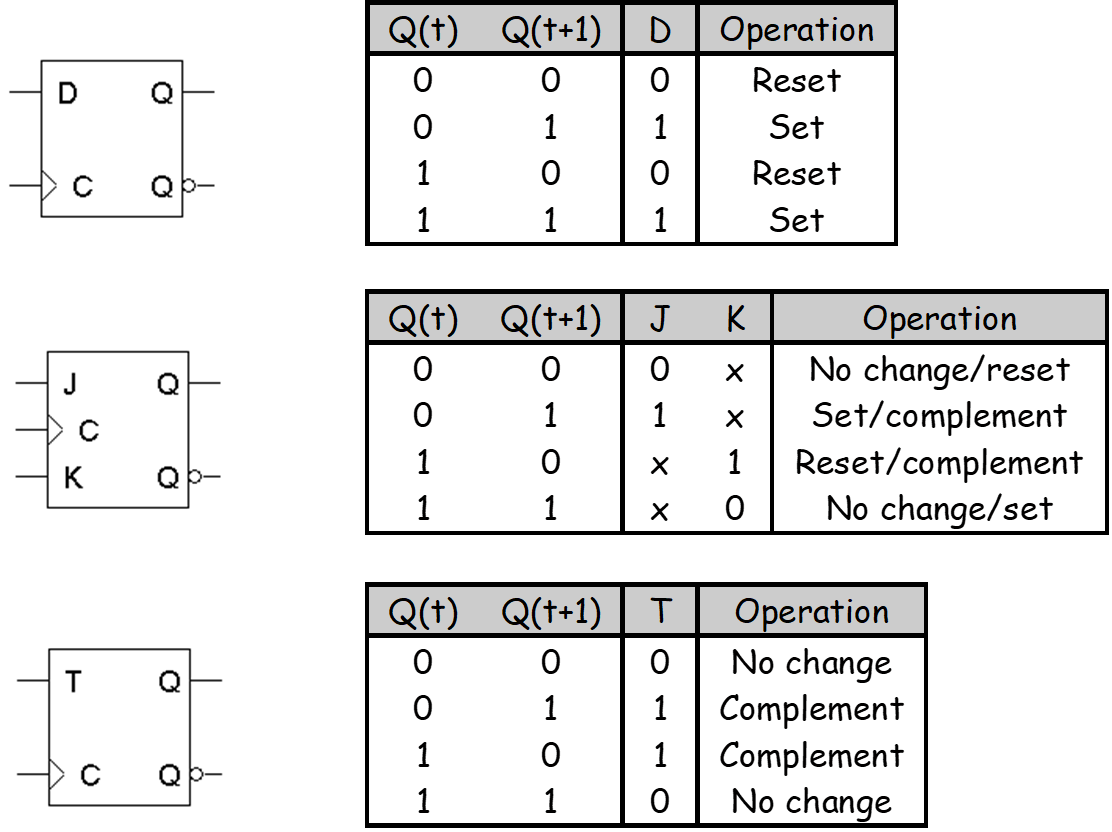
\includegraphics[width=\linewidth]{img/excitation-tables.png}
  \caption{Excitation Tables of Flip-Flops}
  \label{fig:excitation-tables}
\end{figure}

Remember the analysis steps:
\begin{itemize}
  \item Circuit diagram is given
  \item Output and next state equations
  \item State table
  \item (optional) description of what the circuit does.
\end{itemize}
Design is going through the above steps in the reverse order.

\subsection{Sequential Circuit Design Procedure}
\label{subsec:seq-circ-design-procedure}

\begin{enumerate}[label=Step\ \arabic*:, leftmargin=*]
  \item Make a state table based on the problem statement. The table should show the \textit{present states}, \textit{inputs}, \textit{next states} and \textit{outputs}. (\textit{It may be easier to find a state diagram first, and then convert that to a table.})
  \item Assign binary codes to the states in the state table (if you haven't already). If you have $n$ states, your binary codes will have at least $\lceil \log_2 n \rceil$ digits, and your circuit will have at least $\lceil \log_2 n  \rceil$ flip-flops.
  \item For each flip-flop and each row of your state table, find the flip-flop input values that are needed to generate the next state from the present state. You can use flip-flop excitation tables here.
  \item Find simplified equations for the flip-flop inputs and the outputs.
  \item Build the circuit!
\end{enumerate}

\subsection{Example: Sequence Recognizer}
\label{subsec:example-seq-recozginer}

A sequence recognizer is a special kind of sequential circuit that looks for a special bit pattern in some input. The recognizer circuit has only one input, $X$. One bit of input is supplied on every clock cycle. There is one output, $Z$, which is 1 when the desired pattern is found. 

Consider an example that the sequence recognizer will detect the bit pattern ``1001'':
\begin{align*}
  Input&:\quad 1\ 1\ 1\ 0\ 0\ 1\ 1\ 0\ 1\ 0\ 0\ 1\ 0\ 0\ 1\ 1\ 0\ \ldots\\ 
  Output&:\quad 0\ 0\ 0\ 0\ 0\ 1\ 0\ 0\ 0\ 0\ 0\ 1\ 0\ 0\ 1\ 0\ 0\ \ldots
\end{align*}
This requires a sequential circuit because the circuit has to ``remember'' the inputs from previous clock cycles, in order to determine whether or not a match was found. Here, one input and one output bit appear every clock cycle. Note that overlapping bit patterns are also detected (2nd and 3rd instances).

Remember how the state diagram arrows correspond to rows of the state table:
\begin{figure}[H]
  \centering
  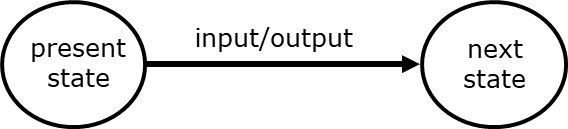
\includegraphics[width=.5\linewidth]{img/design-example-state-diagram-0.png}
\end{figure}

\subsubsection{Step 1: State Diagram (and Table)}
\label{subsubsec:step1-state-diagram-table}

What state do we need for the sequence recognizer?
\begin{itemize}
  \item We have to ``remember'' inputs from previous clock cycles.
  \item For example, if the previous three inputs were 100 and the current input is 1, then the output should be 1.
  \item In general, we will have to remember occurrences of parts of the desired pattern - in this case, 1, 10, and 100.
\end{itemize}

\begin{figure}[H]
  \centering
  \begin{minipage}{\linewidth}
    \centering
    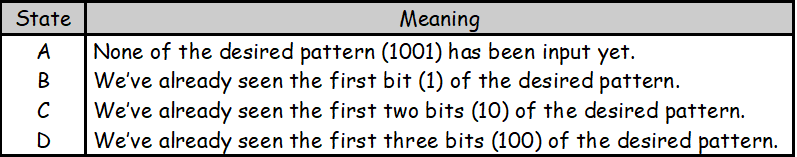
\includegraphics[width=\linewidth]{img/desing-example-table.png}
  \end{minipage}
  \begin{minipage}{\linewidth}
    \centering
    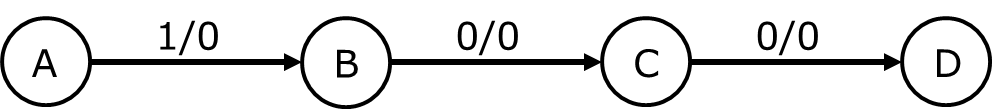
\includegraphics[width=\linewidth]{img/design-example-state-diagram.png}
  \end{minipage}
\end{figure}

What happens if we're in state D (the last three inputs were 100), and the current input is 1?
\begin{itemize}
  \item The output should be a 1, because we've found the desired pattern.
  \item But this last 1 could also be the start of another occurrence of the pattern! For example, 1001001 contains two occurrences of 1001.
  \item To detect overlapping occurrences of the pattern, the next state should be B.
\end{itemize}
\begin{figure}[H]
  \centering
  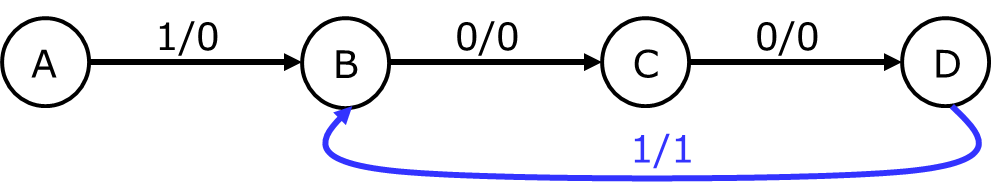
\includegraphics[width=.85\linewidth]{img/design-example-state-diagram-2.png}
\end{figure}

Remember that we need two outgoing arrows for each node, to account for the possibilities of $X = 0$ and $X = 1$. They also allow for the correct detection of overlapping occurrences of 1001.
\begin{figure}[H]
  \centering
  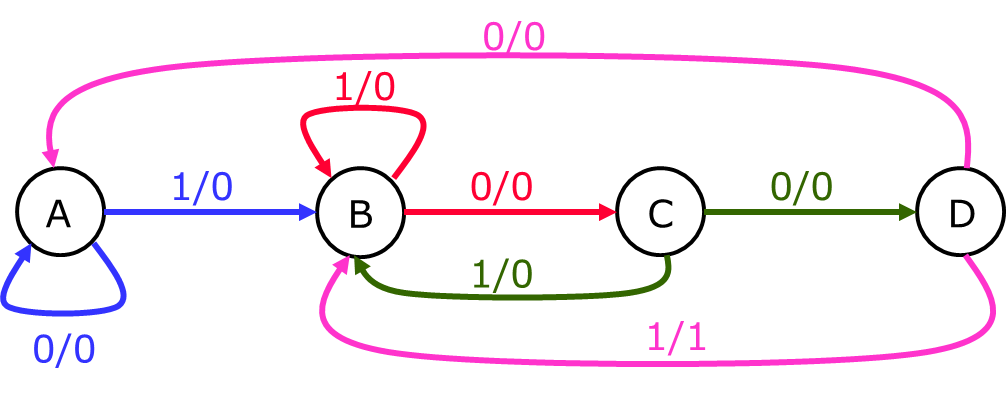
\includegraphics[width=\linewidth]{img/design-example-state-diagram-4.png}
\end{figure}
\noindent Finally, making the state table.
\begin{figure}[H]
  \centering
  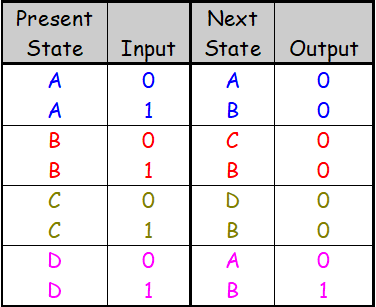
\includegraphics[width=.8\linewidth]{img/desing-example-state-table.png}
\end{figure}

\subsubsection{Step 2: Assigning Binary Codes}
\label{subsubsec:step2-assign-bin-code}

We have four states ABCD, so we need at least two flip-flops $Q_1Q_0$. The easiest thing to do is represent state A with $Q_1Q_0 = 00$, B with 01, C with 10, and D with 11 (intuitive).
\begin{figure}[H]
  \centering
  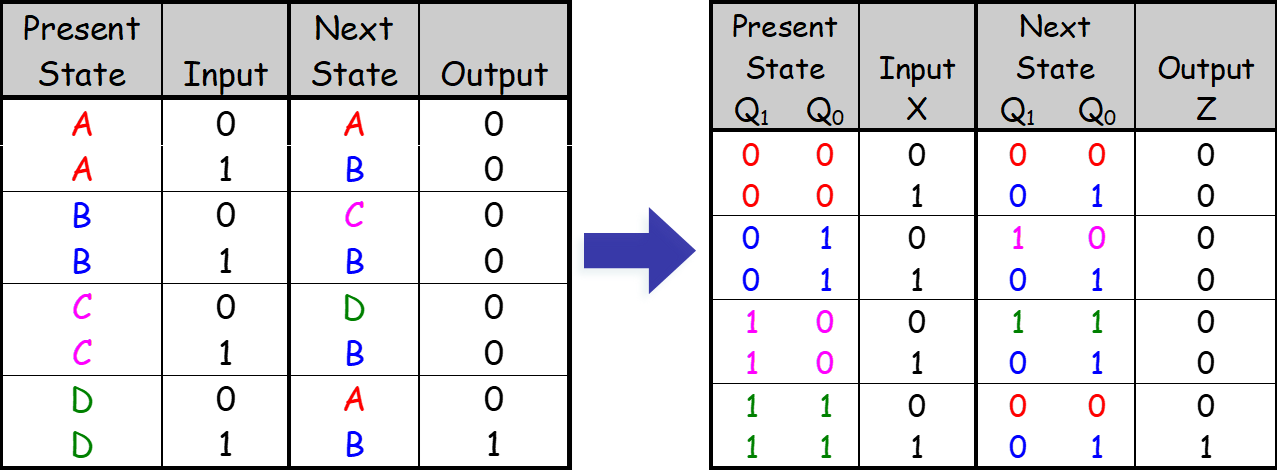
\includegraphics[width=\linewidth]{img/desing-example-state-table-2.png}
\end{figure}

\subsubsection{Step 3: Finding Flip-Flop Inputs}
\label{subsubsec:step3-finding-ff-inputs}

Next we have to figure out how to actually make the flip-flops change from their present state into the desired next state. This depends on what kind of flip-flops you use! We'll use two $JK$s. For each flip-flip $Q_i$, look at its present and next states, and determine what the inputs $J_i$ and $K_i$ should be in order to make that state change.

While doing this, we can use excitation table of $JK$ flip-flop. For example, if the present state of a JK flip-flop is 0 and we want the next state to be 1, then we have two choices for the JK inputs: $JK = 10$ or $JK = 11$.
\begin{figure}[H]
  \centering
  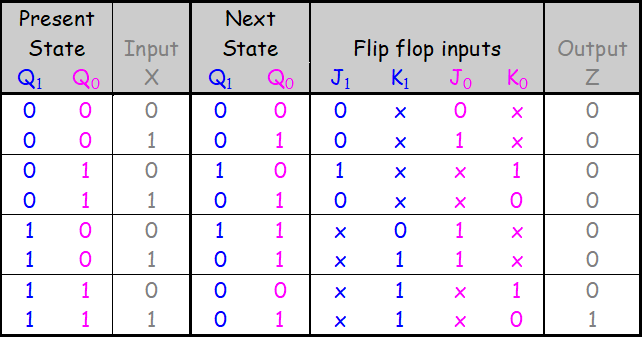
\includegraphics[width=\linewidth]{img/desing-example-state-table-3.png}
\end{figure}

\subsubsection{Step 4: Find Flip-Flop In/Out Equations}
\label{subsubsec:step4-find-ff-io-equations}

Now one can make K-maps and find equations for each of the four flip-flop inputs, as well as for the output $Z$. These equations are in terms of the present state and the inputs. The advantage of using $JK$ flip-flops is that there are many don't care conditions, which can result in simpler equations. In the end, the following equations can be found:
\begin{align*}
	J_0 &= X + Q_1\\
	K_0 &= X'\\
  &\\
  J_1 &= X'Q_0\\
	K_1 &= X + Q0\\
  &\\
	Z &= Q_1Q_0X
\end{align*}

\subsubsection{Step 5: Build the Circuit}
\label{subsubsec:step5-build-the-circuit}

Lastly, we use these simplified equations to build the completed circuit.
\begin{figure}[H]
  \centering
  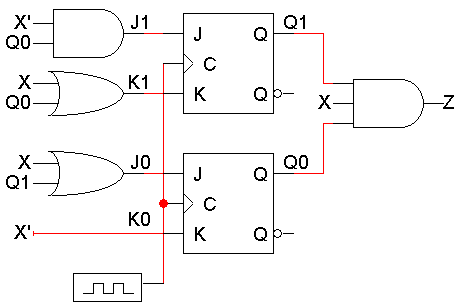
\includegraphics[width=\linewidth]{img/design-example-circuit.png}
\end{figure}
